\documentclass{proc}

\usepackage[margin = 2cm]{geometry}
\usepackage{multirow}

\usepackage{graphicx}
\graphicspath{{graphics/}}

\usepackage{caption, subcaption}

\title{ More on Floats Graphics and Tables}
\author{Tajib Smajlovic}
\date{}


\begin{document}
	
	\maketitle
	
	\section{Introduction}
	Here we'll look at more table and graphics formatting
	
	
	\subsection{More on Tables}
	Table~\ref{tab:wrapping} uses text wrapping in the last column.
	
	\begin{table}[htbp]
		\caption{Text Wrapping}
		\begin{center}
			\begin{tabular}{| l | l | p{3cm} |}
				\hline
				CS101 & Java & Programming with Java \\
				CS201 & Languages & Programming language principles\\
				CS301 & Compilers & Principles of compiler design and implementation \\
				\hline
			\end{tabular}
		\end{center}
	\label{tab:wrapping}
	\end{table}
	
	Table~\ref{tab:multi} uses row and column span.
	
	\begin{table}[htbp]
		\caption{Spanning rows and columns}
		\begin{center}
			\begin{tabular}{| l | c | c |}
				& \multicolumn{2}{c|}{Ranges} \\
				\hline
				& X & Y\\
				\hline
				\multirow{3}{*}{Hot} & 7 & 9\\
				& 5 & 9\\
				& 6 & 7\\
				\hline
				\multirow{3}{*}{Cold}& 4 & 7\\
				& 2 & 9\\
				& 3 & 5\\
				\hline
			\end{tabular}
		\end{center}
		\label{tab:multi}
	\end{table}
	
	
	\subsection{More on graphics}
	Both of my graphics are in the graphics folder for the subfigures, Figure\ref{fig:paper} and Figure\ref{fig:page} in Figure~ref{fig:subs}.
	
	\begin{figure}[htbp]
			\centering
			\begin{subfigure}[b]{0.2\textwidth}
				\centering
				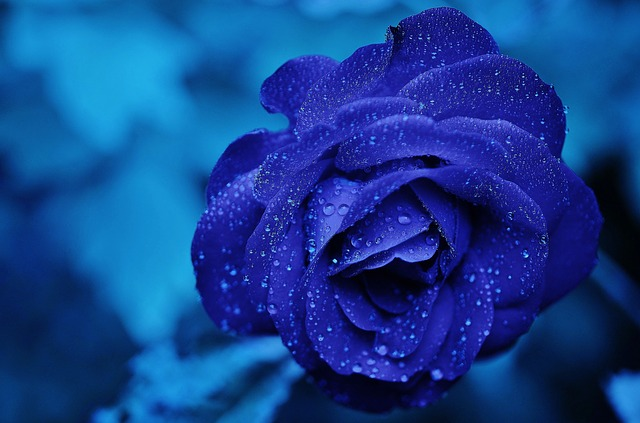
\includegraphics[scale=.1]{one.jpg}
				\caption{Begining}
				\label{fig:paper}
			\end{subfigure}
			\centering
			\begin{subfigure}[b]{0.2\textwidth}
				\centering
				
\includegraphics[scale=.3]{two.png}
				\caption{End}
				\label{fig:page}
			\end{subfigure}
			\caption{The process}
			\label{fig:subs}
	\end{figure}
	
	\section{Conclusion}
	
	
\end{document}